\documentclass[12pt]{article}
\usepackage[utf8]{inputenc}
\usepackage[margin=1in]{geometry}

%Standard Commands
\newcommand{\R}{\mathbb{R}}
\newcommand{\Q}{\mathbb{Q}}
\newcommand{\Z}{\mathbb{Z}}
\newcommand{\N}{\mathbb{N}}
\newcommand{\M}{\mathbb{M}}
\newcommand{\eps}{\varepsilon}
\newcommand{\bs}{\backslash}

%Standard Packages TODO: Figure out what each one does
\usepackage{amssymb}
\usepackage{amsthm}
\usepackage{xcolor}
\usepackage{amsfonts}
\usepackage{graphicx}
\usepackage{float}
\usepackage{amsmath}
\usepackage{version}
\usepackage{caption}
\usepackage{mathtools}
\usepackage{enumerate}
\usepackage{setspace}
\usepackage[parfill]{parskip}

%Standard Theorems
\newtheorem{theorem}{Theorem}
\theoremstyle{definition}
\newtheorem{definition}{Definition}
\newtheorem{example}{Example}
\newtheorem{proposition}{Proposition}
\newtheorem{corollary}{Corollary}
\newtheorem{question}{Question}
\newtheorem{answer}{Answer}

%Doc Info
\title{Volatile Kalman Filter Scaling Law Notes}
\author{Alexander Lanine}
\date{2024-11-25}

\begin{document}
\maketitle

\section*{Introduction}

A central goal for learning theories in psychology and neuroscience is to model how animals and humans learn associations between cues and outcomes. 
Typically, this process is often modeled by updating beliefs based on prediction errors, modulated by a learning rate. 
\textit{Behrens et al.} (2007) proposed that learning rates are dynamically modulated by the \textit{volatility} of the environment: when environmental changes are more frequent, the learning rate should increase, and when changes are less frequent, it should decrease. 
However, the computational model introduced by \textit{Behrens et al.} to describe this relationship is computationally complex and likely not biologically feasible.

To address this, \textit{Piray and Daw} (2020) introduced the \textit{Volatile Kalman Filter} (VKF) as tractable model of learning in volatile environments.
\textcolor{blue}{To Do}

\textbf{Three Parameters:} 
    observation noise $\sigma^2$, initial volatility estimate $v_0$, and volatility update parameter $\lambda$. 

    \begin{enumerate}
        \item Compute Kalman Gain: 
        $$k_t = (w_{t-1}+v_{t-1})/(w_{t-1}+v_{t-1}+\textcolor{blue}{\sigma}^2)$$


        \item Update Posterior Mean:
        $$m_t = m_{t-1} + k_t(o_t-m_{t-1})$$

        \item Update Posterior Variance: 
        $$w_t = (1-k_t)(w_{t-1}+v_{t-1})$$

        \item Update Volatility Estimate: 
        $$v_t = v_{t-1} + \textcolor{blue}{\lambda}
         ((m_t-m_{t-1})^2+w_{t-1}+w_t-2w_{t-1,t}-v_{t-1})$$
    \end{enumerate}

\textcolor{blue}{To Do Introduce Our Findings} 

\newpage 
\section*{Experiment One}

In the first experiment, we assume that the latent state dynamics match are those assumed by the derivation of VKF. That is, that the latent state at time $t$ is given by 
$$s_t = s_{t-1}+e_t,$$
where $e_t$ is a noise term drawn from $\mathcal{N}(0,z_t^{-1}).$ 
The precision $z_t$ is updated according to 
$$z_t = Rz_{t-1}\eps_t,$$
where $R \geq 1$ is a constant and $\eps_t$ is a random variable drawn from a beta distribution governed by 
$$p(\eps_t) = \mathcal{B}(\eps_t \vert \eta\nu, (1-\eta)\nu),$$
where $\eta = R^{-1}$ and $\nu = \frac{1}{2(1-\eta)}$.

First, we run a simulation of the latent state and VKF estimates with parameters: \textcolor{blue}{to do}. 

\begin{figure}[H]
    \centering
    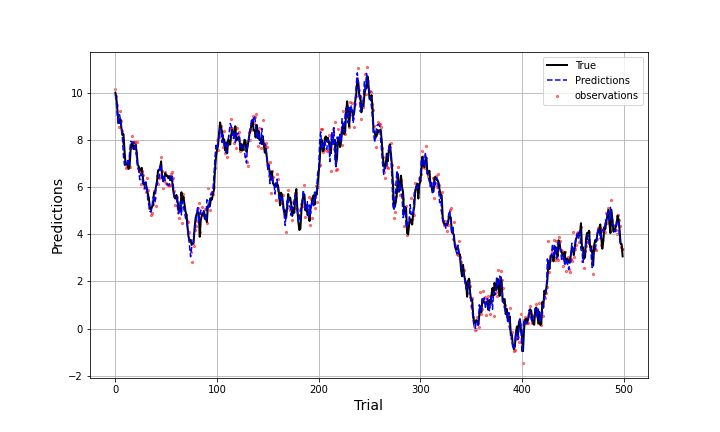
\includegraphics[scale=0.6]{../Figures/exp1_walk.png}
\end{figure}

\begin{figure}[H]
    \centering
    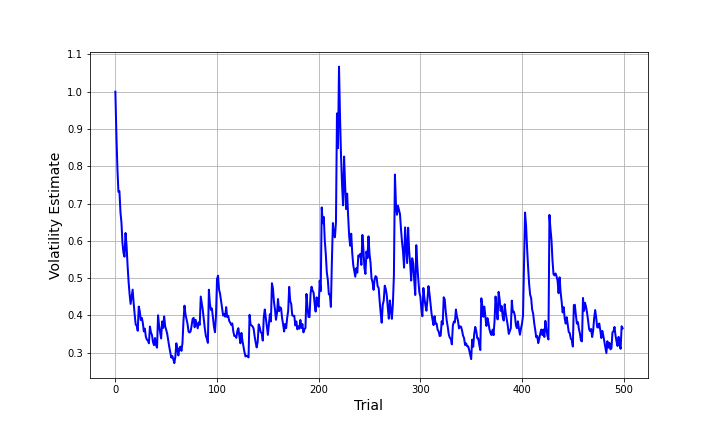
\includegraphics[scale=0.6]{../Figures/exp1_vol.png}
\end{figure}

\begin{figure}[H]
    \centering
    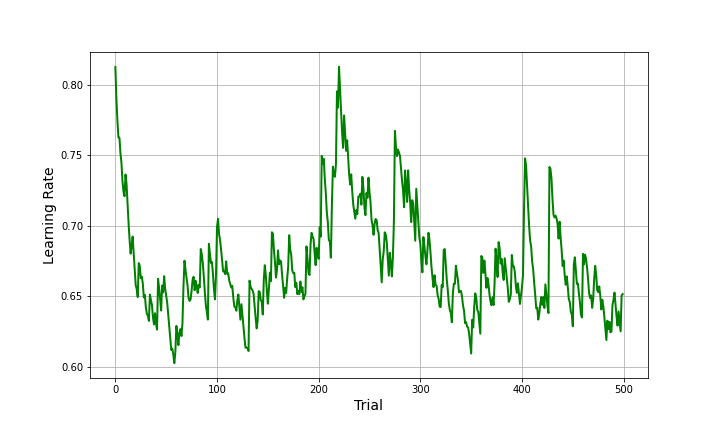
\includegraphics[scale=0.6]{../Figures/exp1_lr.png}
\end{figure}

We now consider the question of how the volatility estimates 


\begin{figure}[H]
    \centering
    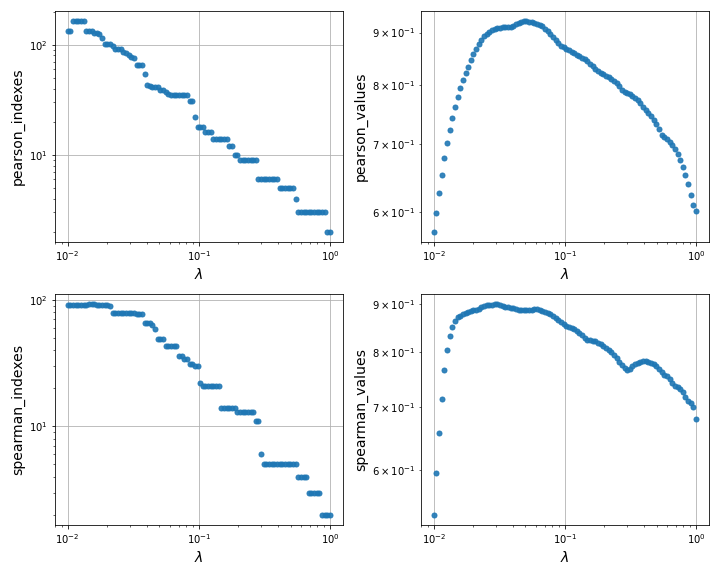
\includegraphics[scale=0.6]{../Figures/exp1_cors.png}
\end{figure}
     

\newpage 
\section*{Experiment Two}
\end{document}